\chapter{Fases en el desarrollo}

\section{Metodología de desarrollo}

Como para inicio de todo proyecto deberemos atender al \textbf{modelo o metodología de desarrollo}. Es aquí donde toma más peso la ingeniería de ``software''\cite{ing_software} estableciendo una metodología formal, con resultados predecibles por las fases de planificación que permitan desarrollar un producto de alta calidad que cumpla las espectativas del cliente. 

Para esta aplicación vamos a elegir un modelo de desarrollo clásico o en cascada\cite{modelo_desarrollo}. Las principales ventajas e incovenientes de este modelo son:

\begin{itemize}
\item [\textbf{Ventajas}]
\item Propicio para proyectos maduros y bien especificados por parte del cliente que no necesitan de mucha investigación para garantizar el desarrollo de los objetivos.
\item Modelo secuencial, en su mayoría, fácil de organizar y entender.
\item Modelo muy extendido y utilizado.
\item Promueve una metodología de trabajo efectiva: definir antes de diseñar, diseñar antes de codificar
\item [\textbf{Inconvenientes}]
\item En el entorno ``cliente-desarrollador'' rara vez el proyecto sigue etapas secuenciales bien definidas, el proyecto va madurando a medida que se va desarrollando, lo cual lo hace ineficaz con este modelo de desarrollo.
\item Tiempo de desarrollo hasta una versión funcional alto ya que no se buscan prototipos intermedios, el desarrollo finaliza una vez terminado y probado.
\item Cualquier error de diseño detectado después de su etapa correspondiente conduce al rediseño y nuevo desarrollo de las etapas afectadas, lo que incremente los costos del desarrollo.
\item Una etapa no se puede iniciar si no se ha terminado la anterior, lo que perjudica a equipos de desarrollo donde cada parte se encarga de una etapa.
\end{itemize}



\begin{figure}[!h]
  \begin{center}
  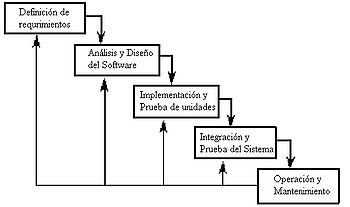
\includegraphics[width=1\textwidth]{../images/modelo_cascada.jpg}
  \caption[Modelo cascada]{ Modelo clásico o de cascada }
  \label{fig:modelo_cascada}
  \end{center}
\end{figure}


\bigskip
Ya que nuestro equipo de desarrollo se compone de una única persona y los requisitos del proyecto están bien definidos vamos a adoptar este modelo de desarrollo.


\bigskip
El modelo de cascada se compone de las siguientes fases:

\begin{itemize}
\item \textbf{Análisis de requisitos:} se determinan los objetivos que debe cumplir el ``software'' que cubran las necesidades de los usuarios finales. Se realiza la especificación completa de las funcionalidades del sistema sin entrar en detalles internos.
\bigskip
Por el tipo de modelo de desarrollo secuencial esta primera fase toma especial importancia. Debe quedar claro todo lo que requiere el sistema ya que no se podrán requerir nuevas funcionalidades a mitad del proceso de desarrollo del proyecto.

\item \textbf{Diseño del sistema:} se descompone el problema a resolver y sintetiza en elementos que puedan elaborarse por separado. De esta forma el equipo de trabajo puede optimizar su rendimiento y elaborar las partes no dependientes. Como resultado del diseño del sistema tendremos una descripción de la estructura global del sistema y la especificación de lo que debe hacer cada una de sus partes, así como la relación entre ellas.
\bigskip
Distinguiremos entre diseño de alto nivel y diseño detallado. Con el \textbf{diseño de alto nivel} de ellos se pretende definir la estructura de la solución (después de analizar el problema en la fase anterior) identificando las diferentes partes. En el segundo de ellos, el {diseño detallado} definiremos los algoritmos empleados para el cumplimiento de los requerimientos del cliente y la organización del código para seguir con la implementación.

\item \textbf{Implementación:} en esta fase se traducen los diseños a una solución legible para el sistema. Es la fase donde se se implementa el código fuente a partir de las fases de análisis y diseño. 

\item \textbf{Integración y prueba del sistema: } es la fase donde se ensamblan las diferentes partes implementadas y se comprueba que funcionan correctamente y que cumplen los requisitos tanto funcionales como no funcionales. Si se ha seguido un desarrollo cuidadoso de la fase de análisis y diseño, esta fase no debe de resultar costosa, las pruebas del sistema no deben encaminar a un rediseño, recordar aquí la importancia de la fase de análisis del problema. 

\item \textbf{Despliegue: } una vez integradas las partes del sistema y probadas pasamos a la fase de \textbf{despliegue} en el lugar donde se alojará, este es el entorno de producción. Comprobaremos que las pruebas sobre este entorno se corresponden con los resultados obtenidos en la fase anterior en el entorno de desarrollo. Una vez se compruebe la integridad de la aplicación en este entorno de producción se da por concluido el desarrollo.
\item \textbf{Matenimiento: } se entiende como fase de mantenimiento todo el proceso posterior al despliegue del entorno de producción y es una de las etapas más críticas, ya que un 75\% de los recursos se destinan a partir de esta fase. Suponiendo que el desarrollo de un proyecto medio pueda durar entre uno y dos años, la fase de mantenimiento se podría alargar entre quince y veinte años. 

\bigskip
En esta fase el usuario final hace uso real del sistema en el entorno de producción y es cuando se determina finalmente si el producto satisface las necesidades por las cuales se implementó a lo largo del tiempo.
\end{itemize}

